%!TEX root = ../thesis.tex
%*******************************************************************************
%*********************************** Methods chapter *****************************
%*******************************************************************************

\chapter{Methods}  %Methods

\ifpdf
    \graphicspath{{Methods/Figs/Raster/}{Methods/Figs/PDF/}{Methods/Figs/}}
\else
    \graphicspath{{Methods/Figs/Vector/}{Methods/Figs/}}
\fi


%********************************** %First Section  **************************************
\section{Patient Cohorts} %Section - 1.1 

Multiple patient cohorts were used throughout the thesis and are detailed at the beginning of the sections they are used in. 

\begin{itemize}
    \item SEARCH
    \item BRITROC
    \item OV04
    \item ICON7
\end{itemize}

\section{Chromogenic Immunohistochemistry (IHC)}

\subsection{Sample preparation}
3μm sections of FFPE blocks were cut using a Leica microtome, transferred to a water bath pre-heated to 60${^\circ}$C and collected on a glass slides. The sections were dried over-night at 37${^\circ}$C then baked at 60${^\circ}$C for 1h. 

\subsection{Manual Staining} 
\subsection{OV04/BRITROC}\label{sec:sarwah_staining}
FFPE sections were rehydrated using the Leica Autostainer ST020 by incubating them twice for 10 min in xylene, followed by two 5 min incubations in 100\% ethanol, one 5 min incubation in 70\% Ethanol and finally washing them in water. Antigens were retrieved in a Tris (10 mmol)-EDTA (1mM) buffer (pH 9.2) preheated to 96${^\circ}$C in a water bath. After 1h incubation, slides were cooled in a water bath for 5 min, washed in Milli-Q water for 5 min and incubated in3\%BSA-PBS for 1h in a hydration chamber at room temperature. ImmEdge pen was used to draw a hydrophobic border around the tissue, and 200μl of primary antibody pre-diluted to the desired concentration in 1\%BSA-PBS were added to the sections. Following an overnight incubation in a hydration chamber at 4$^{\circ}$C, the antibody solution was drained and the slides were washed twice for 5 min in 1\% Tween-TBS, succeeded by two washes for 5 min in TBS. For HRP-conjugated primary antibodies, DAB was directly added to the slides. For secondary antibody staining, pre-diluted secondary antibody was added and incubated at room temperature for 30 min, followed by 2 washes in TBS. The slides were incubated in DAB chromogen for
5 min, washed in Milli-Q water, and dehydrated and cover-slipped using the Leica Autostainer ST020.

\subsubsection{SEARCH}
Sectioning and was carried out as following on the SEARCH cohort. Microarray slides composed of FFPE embedded ovarian tumour cores were dewaxed and rehydrated prior to heat induced epitope retrieval (HIER) using a pressure cooker and a citrate-based antigen unmasking solution (Vector Laboratory). Detection of CD8$^+$ T cells, CD45RO$^+$ memory lymphocytes and CD68$^+$ macrophages was performed using the mouse anti-human CD8 (Clone C8/144B, Dako), mouse anti-human CD45RO (Clone UCLH, Dako) and mouse anti-human CD68 (Clone M0876, Dako) antibodies, using ultrasensitive Polymer-HRP IHC Detection system (Biogenex). Immunohistochemical protocols and slide hybridizations were carried out manually. Sections were counterstained with haematoxylin and mounted with DPX mounting medium (Sigma). Stained slides were scanned using the Panoramic Slash Scanner (3D Histech).

\subsection{Automated Staining}
Automated staining was carried out using the Ventana Discovery Ultra platform.  All bulk reagents used were purchased from Roche and are listed in Table \ref{table:bulk_reagents}. The slides were rehydrated by incubating them in EZ prep solution for 32 min at 69${^\circ}$C, then incubated for 1h in VentanaCell Conditioning buffer 1 (CC1) at 96${^\circ}$C for antigen retrieval (pH 8.5). Hydrogen peroxide was then applied and incubated for 4 min to quench endogenous peroxidase activity, followedby primary antibody incubation for 1h at 37${^\circ}$C. Details of antibodies used for chromogenic IHC are listed in Table \ref{table:ihc_antibodies}.  After a16 min incubation with an HRP-conjugated secondary antibody, the chromogenic signal was developed in either 3, 3’-Diaminobenzidine (DAB) chromogen for 8 min, in Purple chromogen for 40 min, in Yellow chromogen for 28 min or in Teal chromogen for 8 mins. For chromogenic counter-staining, the slides were incubated for 4 min in Copper,8 min in haematoxylin and 4 min in Bluing Reagent. Slides were washed with Reaction Buffer after each incubation. As a negative control, Mouse IgG, Rabbit IgG and GoatIgG isotype replaced mouse, rabbit and goat primary antibodies, respectively. Stained slides were dehydrated using the Leica Autostainer ST020, manually cover-slipped and digitally scanned by Aperio Scanscope XT. 
\begin{table}[]
    \centering
    \begin{tabular}{lc}
    \hline
    Reagent & Code \\
    \hline
    EZ prep & 950-102 \\
    Ultra Cell Conditioning Solution (CC1) & 950-224\\
    Ultra Liquid Cover Slip (LCS) & 650-210 \\
    Reaction Buffer & 950-300 \\
    ChromoMap DAB Kit & 760-159\\
    Purple Kit & 760-229 \\
    Yellow Kit & 760-239 \\
    Antibody Diluent & 760-108\\
    Haematoxylin II & 760-2208\\
    Bluing reagent & 760-2037\\
    OmniMap Anti-Ms-HRP Secondary Antibody    & 760-4310\\
    OmniMap Anti-Rb-HRP Secondary Antibody & 760-4311 \\
    \hline
    \end{tabular}
    \caption{Caption}
    \label{table:bulk_reagents}
\end{table}

\section{Imaging Mass Cytometry}
\subsection{Imaging Mass Cytometry (IMC) Antibody purification}
Carrier proteins like bovine serum albumin (BSA) are commonly added to the storage buffer of antibodies as preservatives. These proteins can replace antibodies in the conjugation process,reducing the efficiency of antibody conjugation to metals. Antibodies with carrier proteins were therefore purified using the Pierce™Antibody Clean-up Kit (ThermoFisher, 44600) following the manufacturers instruction.  This involves a desalting step, where the antibody is passed through a Zeba spin desalting column containing a resin bed and centrifuged for 2 min at 1000×g. The antibody is then added to a spin column containing a Purification Support slurry,incubated at room temperature for 5 min with end-to-end mixing, then centrifuged for 1 min at 4000×g to collect the purified antibody.The purity of the antibody was tested using a NuPAGE™4-12\% Bis-Tris Gel (Invitrogen,NP0321BOX). The antibody was mixed with LDS Sample buffer (Invitrogen, NP0007) and Sample Reducing agent (Invitrogen, NP0009) and incubated at 70${^\circ}$C for 10 min. 1μg of the original antibody and the purified antibody were loaded onto the gel, with a BSA-only sample used as a control. The gel was run in Bolt MPOS SDS Running Buffer (Invitrogen, B0001)at 120V for 30 min followed by 2h at 60V. The gel was stained with InstantBlue (Expedeon,ISB1L) to visualise the protein bands, and imaged using Antibody-Metal conjugation Carrier-free antibodies were metal-conjugated using the Maxpar®X8 Antibody Labelling Kits (Fluidigm) according to the manufacturers instructions. A proprietary polymer is loaded with a lanthanide metal by mixing them in the provided L-buffer and incubating them in a 37${^\circ}$C water bath for 35 min. The metal-loaded polymer is filtered to remove excess metal by centrifuging it twice in a 30kDa Amicon Ultra500 μlV bottom (Millipore, UFC505096) at 14,000×g for a total of 55 min. The antibody is centrifuged at 14,000×g in a 50kDa AmiconUltra500 μlV bottom (Millipore,  UFC505096) for 10 min,  and then partially reduced by incubating it in 4mM PierceTM Bond-Breaker®TCEP Solution (ThermoFisher Scientific,77720) at37${^\circ}$C for 30 min.  This is immediately followed by three washes in the provided C-buffer, with a 10 min centrifugation at 14,000×g after each wash. The metal-loaded polymer is added to the partially reduced antibody and incubated in a 37${^\circ}$C water bath for 90 min.The metal conjugated antibody is washed four times in the provided W-buffer, with a 10 min centrifugation at 14,000×g after each wash. The antibody is finally suspended in 100μl PBS containing 0.05\% sodium azide as a preservative, and collected by centrifuging the inverted filter in a fresh microcentrifuge tube for 2 min at 1,000×g. The concentration of the antibody was measure using NanoDrop Spectrophotometer ND-1000 (LabTech International).

\subsection{Staining and Imaging}
The manual staining  protocol outlined in  section \ref{sec:sarwah_staining} was also followed for IMC.  Metal-conjugated primary antibodies were used instead of unconjugated or HRP-conjugated antibodies. Details of all antibodies used are displayed in Table \ref{table:imc_antibodies}.
\begin{table}[]
    \centering
    \begin{tabular}{lllllc}
    \hline
    Antigen & Clone & Tag & Source & Code & Concentration() \\
    \hline
    CA9 & polyclonal & 141Pr & Novus & BioAF2188 & 2  \\
    p53 & DO-7 & 143Nd & Fluidigm & 3143026D & 5 \\
    CD16 & EPR16784 & 146Nd & Fluidigm & 3146020D & 10\\
    CD163 & EDHu-1 & 147Sm & Fluidigm & 3147021D & 5 \\
    PanK & C11 & 148Nd & Fluidigm & 3148020D & 1 \\
    CD56 & MRQ-42 & 151Eu & Cell Marque & 156R-96 & 1 \\
    CD45 & D9M8I & 152Sm & Fluidigm & 3152018D & 1.5\\
    LAG3 & D2G40 & 153Eu & Fluidigm & 3153028D & 2.5\\
    TIM3 & D5D5R & 154Sm & Fluidigm & 3154024D& 2.5\\
    FoxP3 & 236A/E7 & 155Gd & Fluidigm & 3155016D & 5\\
    CD4 & EPR6855  & 156Gd & Fluidigm & 3156033D & 5\\
    CD68 & KP-1 & 159Tb & Fluidigm & 3159035D & 2\\
    PD1  & D4W2J & 160Gd & Cell Signalling & 86163S & 5 \\
    CD20 & H1 & 161Dy & Fluidigm & 3161029D & 5\\
    CD8 & aC8/144B & 162Dy & Fluidigm & 3162034D & 5\\
    CD103 & EP206 & 163Dy & Cell Marque & 437R-16 & 3\\
    CK7 & RCK105 & 164Dy & Fluidigm & 3164028D & 10\\
    pH2AX & N1431 & 165Ho & Fluidigm & 3165036D & 0.5\\
    B7h4 & D1M8I & 166Er & CST14572 & 5 \\
    GranzymeB & EPR20129-217 & 167Er & Fluidigm & 3167021D & 1 \\
    Ki67 & B56 & 168Er & Fluidigm & 3168022D & 1.5\\
    Collagen 1 & Polyclonal & 169Tm & Fluidigm & 3169023D & 1\\
    CD3 & Polyclonal & 170Er & Fluidigm & 3170019D & 7.5\\
    CTLA4 & BSB88 & 171Yb & BioSB & BSB 2885 & 7.5\\
    OX40 & ACT-35 & 172Yb & CST98785 & 5\\
    CD45RO & UCHL1 & 173Yb & Fluidigm & 3173016D & 3\\
    HLADR & TAL 1B5 & 174Yb & ThermoFisher & MA1-46109  & 0.5\\
    ICOS & D1K2T & 175Lu & CST & 3148021D & 5\\
    Histone H3 & D1H2 & 176Yb & Fluidigm & 3176023D & 0.25\\
    Intercalator &  & 191Ir, 193Ir  & Fluidigm  & 201192A & 1:1000\\
    \hline
    \end{tabular}
    \caption{IMC antibodies}
    \label{table:imc_antibodies}
\end{table}
Following the two washes in 1\% Tween-TBS and two washes in TBS, the slides were counter-stained with Cell-ID™Intercalator-Ir for 30 min at room temperature. The slides were then washed in Milli-Q water for 5 min, and air dried for at least 20 min before imaging on the Hyperion™Imaging System(Fluidigm). Images were acquired using a UV laser at a frequency of 200 Hz. Metals in each pixel ablated were plasma-ionised and their count was detected using Cytometry by Time of Flight (CyTOF) technology. This was used to generate a stack of false-colour images, each layer corresponding to a single metal and the intensity of each pixel reflects the amount of each antigen present. 

\subsection{Image analysis}
Python was used for data cleaning and applying median filters.

Imagej was used for analysis of collagen structure.

QuPath was used for classification of individual cells from H&E and Cytokeratin images.

Definiens was used for the classification of SEARCH.  Definiens image analysis algorithms for detection of epithelial and stromal areas were trained and the segmentation for each core was manually refined by AM and a consultant gynaecological-histopathologist (J. McD.).

Analysis of images taken from both chromogenic IHC and IMC was done using the HALO Image Analysis Platform (Indica labs). Halo was used for tissue classification and immune cells identification and extraction in SEARCH, BRITROC and OV04. 

%********************************** % Fourth Section  *************************************
\section{Statistical Analysis}  %Section - 1.4
\label{section1.4}

R (version 3.5.1) was used for statistical analysis and R markdown documents are provided in Supplementary Methods that reproduce all results. All count data were transformed to log base 10 after adding a small offset to zero values. Wilcoxon signed rank test was used to compare the mean infiltrate between groups. Continuous data were presented as median and interquartile range (IQR) and groups were compared by the Kruskal–Wallis and pairwise Kruskal-Wallis tests. Discrete data were presented as count and percentage.  

The functional form of immune variables was assessed using comparison with cubic splines. The best approximations to the functional forms were carried forward for the Cox models. 

I carried out quality assurance tests for spatial bias across TMAs and investigated the sources of varying tissue area visually using heatmaps and statistically using Shapiro-Wilk tests.


\subsection{Survival Analysis}

Cox regression was used to examine the relationship between predictors $X$ and the hazard.

The hazard function is given by the following formula:
\begin{equation}H(t) = H_0(t) e^ {b_1 X_1 + ... + b_n X_n} \end{equation} 

Where $H$ is the hazard, the predictors are denoted $X_n$ and Cox regression estimates the coefficients of the predictors $b_n$. The proportional hazard model is semi-parametric as there is an assumption that the hazard is a linear function of the predictors and that the hazards are proportional (the coefficients are not a function of time). There are no assumptions about the form of the baseline hazard function $H_0(t)$. 

The Akaike Information Criterion (AIC), equation \ref{eq:AIC} as detailed in the Methods, was used to compare the performance of survival models, which includes the loglikelihood of the model $\hat{L}$ and a penalty on the number of terms, $k$ to reduce overfitting. 

\begin{equation}
\label{eq:AIC}
    {\displaystyle \mathrm {AIC} \,=\,2k-2\ln({\hat {L}})}
\end{equation}

\subsection{Spatial Statistics}

Spatial statistics can most easily be carried upon 2D point patterns. In such analyses cells are assumed to be points with coordinates $(x,y)$ and zero radius $r=0$. The value of the center of the point for each cell is given in equation \ref{eq:1}. 

\begin{equation}    x=\frac{x_{max} + x_{min}}{2}        y = \frac{y_{max} + y_{min}}{2}
\label{eq:1}
\end{equation}
We will see that these assumptions are violated but information can still be gleaned from these measurements as long as the consequences and limitations of such assumptions are understood.

\subsection{Density based analysis}

\subsubsection{Global density}
The simplest measure of the density of a point pattern is the following:
\begin{equation}
    \lambda = \frac{n}{|A|}
\end{equation}
Where $\lambda$ is the number of points in a region and $A$ is the area measure of the region. 

\subsubsection{Ripley's K function}
Ripley's K function measures the distribution of points within a certain radius and is defined as:
\begin{equation}
K(r)=\lambda^{-1}E
\end{equation}
Where $\lambda$ is the density and $E$ is the expected number of points in the region.

\subsubsection{DBSCAN}
DBSCAN stands for Density based clustering. There are many clustering methods in existence but when clustering spatial data rather than data in information space, DBSCAN has been shown to be best at clustering groups\cite{}.

\subsection{Distance based analysis}

\subsubsection{k-nearest neighbour}
k-nearest neighbour method derives for each point in a point pattern, the $k^{th}$ nearest neighbour to it.
The theoretical expected distance \ref{eq:knn} to the nearest neighbour in a random 2D point pattern is derived as follows;

\begin{equation}
    
\end{equation}

\begin{equation}
\label{eq:knn}
    <r_n> = \frac{1}{2\sqrt{\lambda}}
\end{equation}
Where $\lambda$ is the global density of points.


\begin{figure}
    \centering
    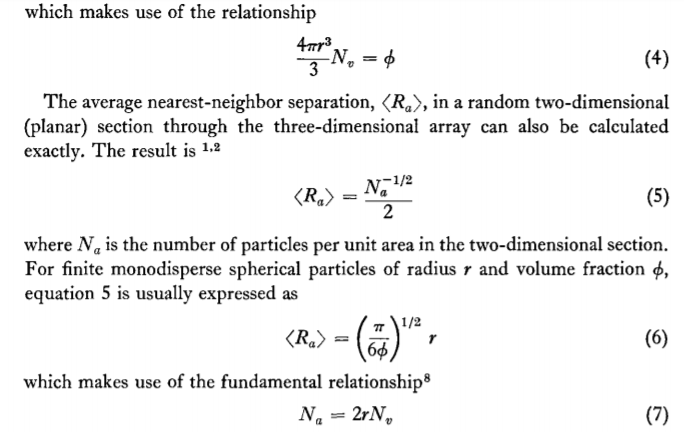
\includegraphics{Chapter3/Figs/knn.PNG}
    \caption{Add these equations to describe distances}
    \label{fig:knnequations}
\end{figure}

\subsection{Intensity analysis}

The Grey Level Co-occurence Matrix (GLCM)\cite{GLCM} measures texture features based on pixel intensities.
These include the following:

\subsubsection{Entropy}
Entropy is a measure of information mixing. Increasing disorder increases entropy. Shannon entropy is defined as \begin{equation}
    H = \sum_{i=1} {p_i log p_i}
\end{equation}

Where $p_i$ is the probability of obtaining class $p$.

Entropy can be defined on an image or image region based on pixel grayscale values.